%%%%%%%%%%%%%%%%%%%%%%%%%%%%%%%%%%%%%%%%%%%%%%%%%%%%%%%%%%%%%%%%%%%%%%
% How to use writeLaTeX: 
%
% You edit the source code here on the left, and the preview on the
% right shows you the result within a few seconds.
%
% Bookmark this page and share the URL with your co-authors. They can
% edit at the same time!
%
% You can upload figures, bibliographies, custom classes and
% styles using the files menu.
%
%%%%%%%%%%%%%%%%%%%%%%%%%%%%%%%%%%%%%%%%%%%%%%%%%%%%%%%%%%%%%%%%%%%%%%

\documentclass[12pt]{article}
\usepackage[brazil]{babel}
\usepackage[pdftex]{hyperref}
\usepackage[table,xcdraw]{xcolor}
% \usepackage[numbers]{natbib}


\usepackage{sbc-template}
\usepackage{listings}

\usepackage{graphicx,url}

\usepackage[utf8]{inputenc}  
\usepackage{float}
\sloppy

\title{Sistema de controle e monitoramento para LEDs em tempo real usando Web App e Firebase}

\author{João Vitor Moreira Duarte }

\address{Instituto de Federal de Educação e Tecnologia -- Campús do Maracanaú
  (IFCE)\\
  Av. Parque Central, 1315 - Distrito Industrial I, Maracanaú - CE, 61939-140
  \email{joao.vitor.moreira08@aluno.ifce.edu.br}
}

\begin{document}

\maketitle
\begin{abstract}
  Nowadays, it is very common to come across the automation of hunting
  sas, with this project I demonstrate a form of smart lamps in a
  small-scale and low-cost means of demonstration. Using of
  LEDs and an ESP32 communicating with a web application, it is possible to control
  the states of the lights.
\end{abstract}
\begin{resumo}
  Nos dias atuais é muito comum se deparar com a automação de casas, com esse projeto demonstro uma forma
  de lampadas inteligentes em uma escala reduzida e de baixo custo para meios de demonstração. Utilizando de LEDs
  e um ESP32 comunicando com uma aplicação web, é possível controlar os estados das luzes.
\end{resumo}

\section{Introdução}

\emph{Smart Home}, que, em tradução direta significa Casa Inteligente, é um conceito
que envolve varias éreas de conhecimento da ciência e engenharia. Este termo é
comumente utilizado para definir uma residência que integra tecnologia e serviços através de
uma rede com o objetivo de aprimorar a eficiência energética e melhorar a qualidade de vida.\cite{MULANI}.
Logo uso de microcontroladores para controlar lampadas é uma forma de deixar a residencia inteligente.

Segundo \cite{ALMEIDA} a automação residencial ainda possui um alto custo para o
grupo ao qual se destina. Tendo em vista que nem todos tem acesso a grandes orçamentos para tentar automatizar sua residencia,
é de grande importância que seja possível criar soluções baixo custo quando pensamos em automatizar alguma parte do dia a dia dentro de uma residencia.

Dessa forma projetos como controle de LEDs com Web App, simples e de custo baixo são uma boa porta de entrada para uma casa mais automatizada,
assim utilizando o microcontrolador ESP32 que tem um custo relativamente baixo comparado com um gerenciador de casa inteligente como uma Alexia da
Amazon ou um Google Nest da própria Google é possível deixar uma residencia mais \emph{smart} sem grandes custos e com controle maior da privacidade dos seus dados.

\section{Fundamentação Teórica}
Para esse projeto foi levado em consideração a assediabilidade para reprodução, dessa forma o projeto visa utilizar somente de softwares gratuitos e materiais de baixo custo.
Com isso, usaremos somente o microcontrolador ESP32 pelo seu preço acessível e sua capacidade de conectar-se a uma rede sem fio, para fazer a comunicação entre usuário e
controlador sera feito uso de uma pagina web e um conjunto de serviços ofertados pelo Firebase. E para ambiente de desenvolvimento,
sera utilizado o Arduino IDE, que é uma ferramenta para programar placas como o ESP, Arduino e raspberry's.

\section{Materiais e Serviços}
Para esse trabalho, pode se dividir o sistema completo em construção do sistema de acionamento de LEDs usando o somente o ESP32, três LEDs e três resistores,
junto dos serviços de \emph{hosting, realtime database} e autenticação ofertados pelo Firebase o \emph{Backend as a Service} da Google por ter ser tier gratuito.

\subsection{ESP32}
De acordo com \cite{EXPRESSIF} ESP32 é um módulo microcontrolador (MCU) Wi-Fi, \emph{Bluetooth}, \emph{Bluetooth Low Energy}(BLE), de ampla variedade de aplicações,
desde de redes de sensores de baixa potência a tarefas mais exigentes, como codificação de voz, streaming de música e decodificação de MP3.

Nesse projeto ele vai servir como controlador primário dos LEDs conectados.

\subsection{Arduino IDE}
É uma aplicação de plataforma cruzada, escrito em funções de C e C ++. É usado para escrever e fazer upload de
programas em placas compatíveis com Arduino, mas também, com a ajuda de núcleos de terceiros, outras placas de
desenvolvimento de fornecedores.

\subsection{Web App}
O Web App é nossa sera praticamente o 'rosto' da aplicação aonde o usuário poderá fazer seu login e a partir disso controlar os estados de cada Led.
Para seu desenvolvimento foi usado html, css e javascript. Sendo a parte da aplicação responsável por criar a ponte entre o usuário e o controlador dos LEDs.

\subsection{Firebase}
Firebase é um \emph{backend as a service}, que tem um conjunto de serviços nos quais iremos utilizar para
facilitar a infraestrutura do projeto. Essa plataforma da Google conta com varias serviços que extremamente
utilizados para criação de qualquer tipo de serviço.

\subsubsection{Authentication}
O Firebase oferta vários tipos de autenticação mas para esse projeto foi utilizado a mais simples, email e senha. Cada usuário que pretende utilizar o sistema deve ser cadastrado para que possa logar no nosso Web App.
\subsubsection{Realtime Database}
De acordo com a sua documentação o \emph{Firebase Realtime Database} é um banco de dados \emph{NoSQL} hospedado na nuvem.\nocite{FIREBASERD}

Assim a principal função é armazenar o estado dos LEDs da protoboard usando como identificação os pinos os quais estão conectados no ESP32.

E para complementar, por ser um serviço de \emph{backend} o Firebase fornece um conjunto de regras que permitem controlar as permissões dentro da aplicação.
Dessa forma foi configurado que o acesso ao banco somente para o usuário cadastrado.
Logo somente ele pode alterar os dados dentro do banco.

\begin{figure}[ht]
  \centering
  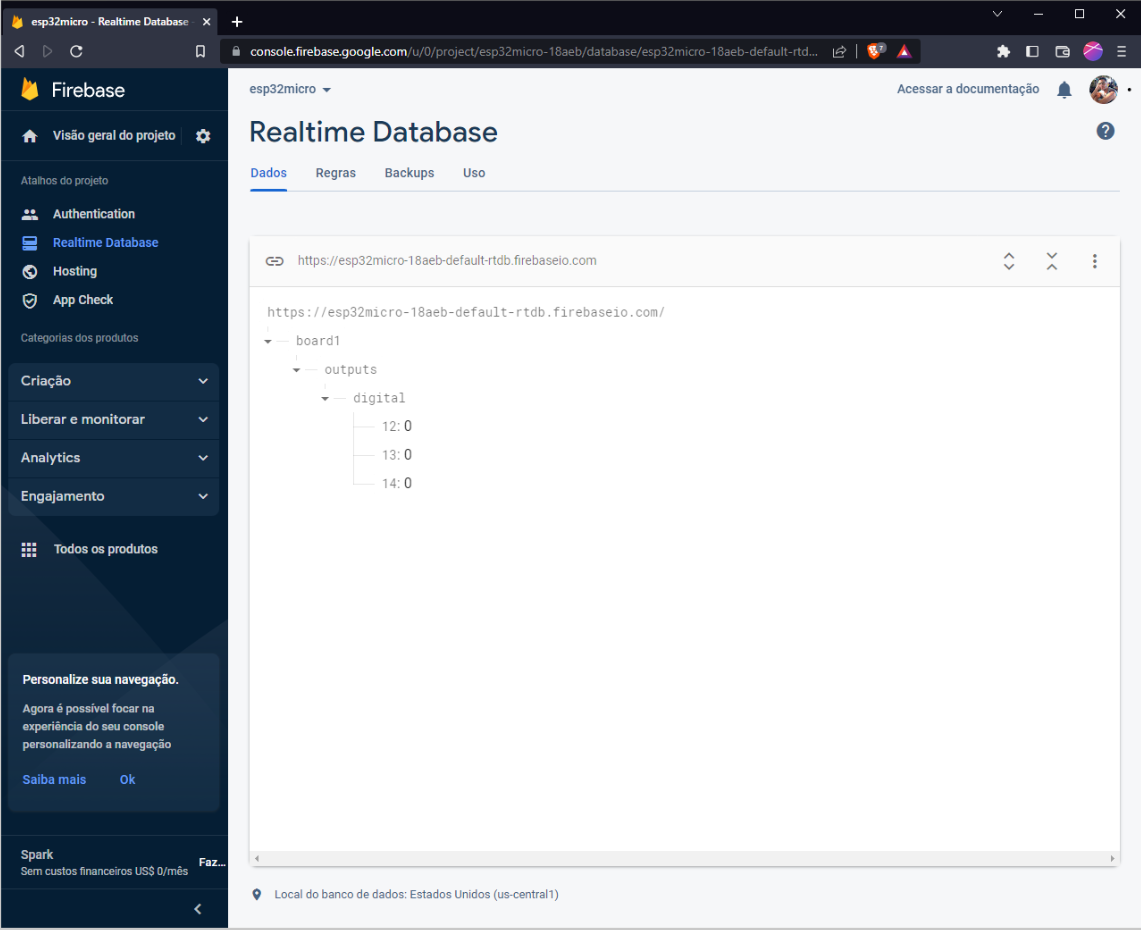
\includegraphics[width=.5\textwidth]{Images/frd3.png}
  \caption{Imagem do banco implementado}
  \label{fig:FirebaseRealtimeDatabase}
\end{figure}

\begin{figure}[ht]
  \centering
  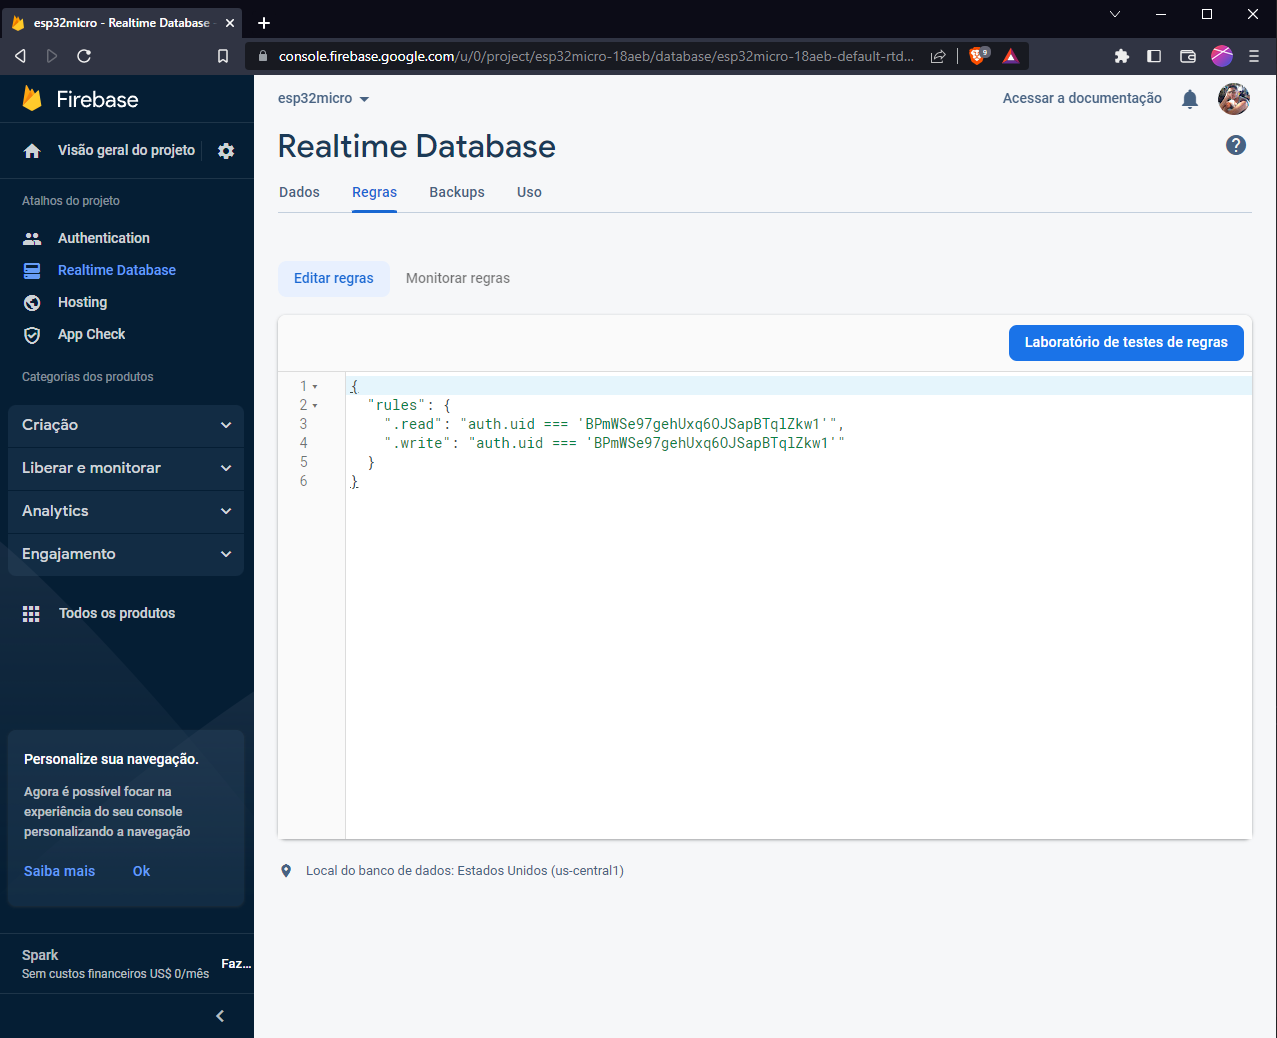
\includegraphics[width=.5\textwidth]{Images/rules.png}
  \caption{Imagem das regras dentro do Firebase}
  \label{fig:FirebaseRules}
\end{figure}

\subsubsection{Hosting}
Com o Firebase, foi possível fazer o deploy da aplicação e já gerar seus próprios urls com domínios fornecidos pela própria plataforma. Simplificando muitos passos de um \emph{deploy} tradicional.

\section{Resultados}
Como resultado final foi obtido um projeto com um \emph{backend} configurado no \emph{Firebase} tendo suporte a autenticação, banco de dados, controle de acesso e até hospedagem. Um  \emph{frontend} feito
com as linguagens da web e um sistema de controle de LEDs em tempo real capaz de funcionar em qualquer dispositivo com acesso a internet.E por fim, sem comprometer a e baixo custo simplicidade
para que seja possível qualquer um replicar os mesmos resultados com baixo orçamento.

Um video demonstrativo pode ser acessado em: \href{https://drive.google.com/file/d/1KFUTW1jYnxYv23ianrwgQhIxSgZv7Ih3/view?usp=sharing}{\ttfamily{aqui.}}

\begin{figure}[!ht]
  \centering
  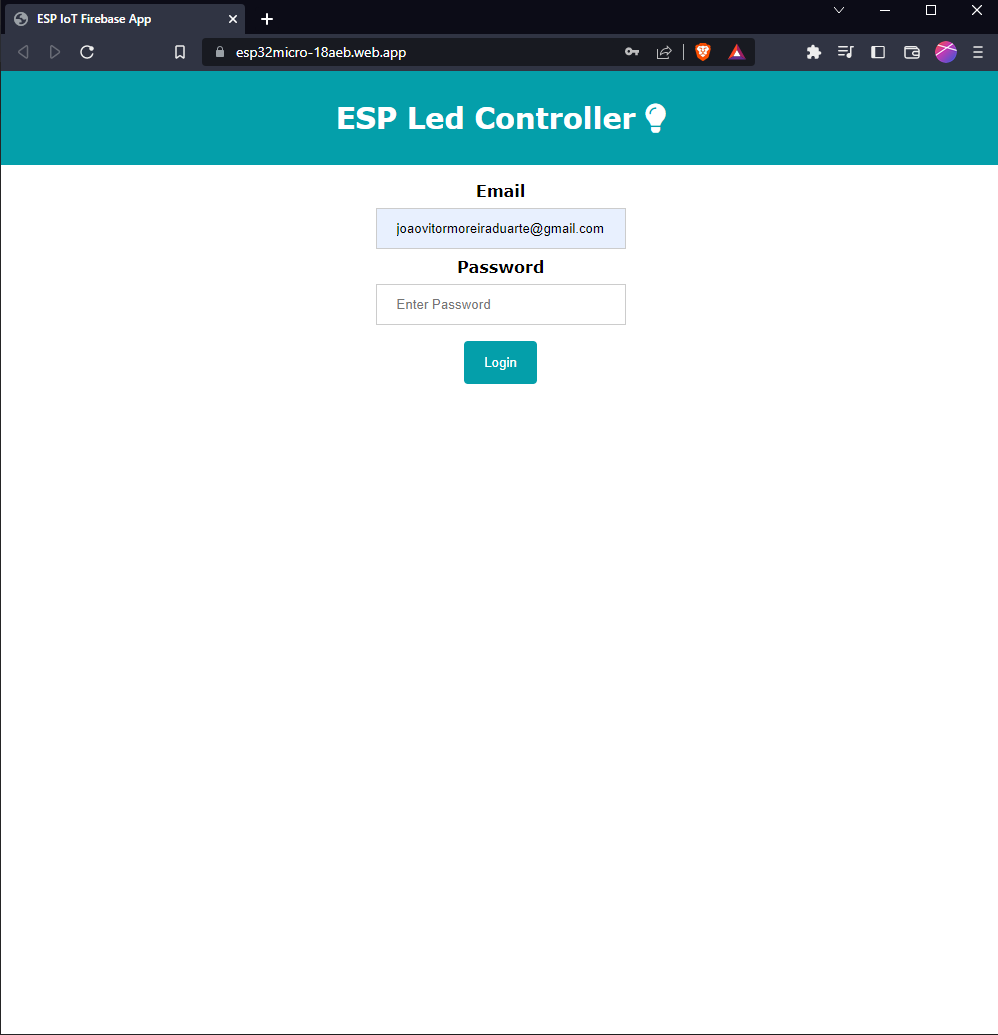
\includegraphics[width=.4\textwidth]{Images/front1.png}
  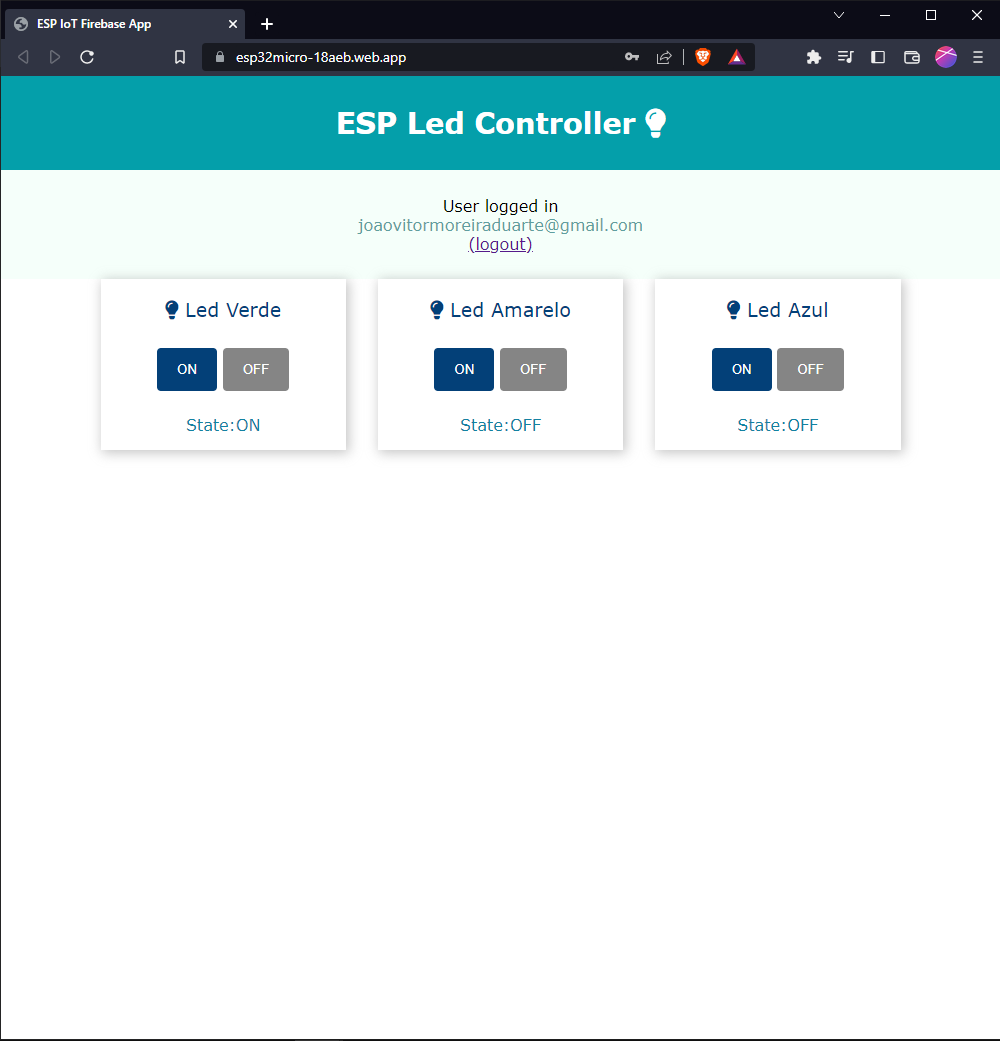
\includegraphics[width=.4\textwidth]{Images/front2.png}
  \caption{Imagem do Web App}
  \label{fig:webAppIllustration}
\end{figure}

\begin{figure}[!ht]
  \centering
  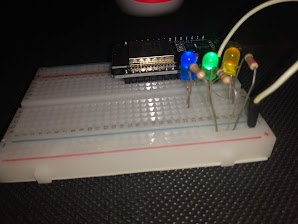
\includegraphics[width=.4\textwidth]{Images/results1.jpg}
  \caption{Imagem do sistema ligado}
  \label{fig:Resultados01}
\end{figure}

\section{Conclusão}
Apesar de algumas dificuldades técnicas causadas pelo ESP32, foi possível implementar todos os passo necessários para criar o ambiente de desenvolvimento
favorável para o sucesso desse projeto.

Ao concluir esse projeto pude aplicar os conhecimentos em programação junto aos de microcontroladores, podendo fazer uma ponte entre eles.
Dessa forma, implementado um protótipo de automação que pode ser aplicado em qualquer residencia e de baixo custo. Para o futuro seria interessante aplicar os conhecimentos obtidos com os testes com LEDs para usar em lampadas
para construir um sistema de automação domiciliar totalmente customizável com rotinas de iluminação.

\bibliographystyle{sbc}
\bibliography{sbc-template}
\end{document}
